\section{Fit-ordered diverse search}
\label{sec:method}

\begin{figure*}[!t]
\centering
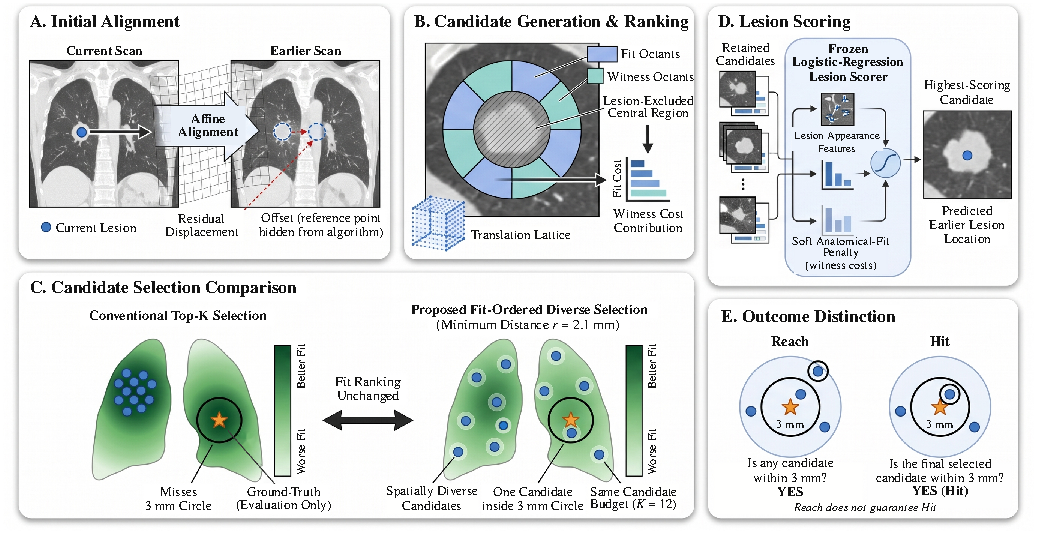
\includegraphics[width=0.8\textwidth]{figures/overview.pdf}
\caption{Method overview. (A)~Chest alignment leaves a residual displacement. (B)~Translations are scored on a shell around the lesion: fit octants give $f_t$, witness octants $w_t$. (C)~At the same budget, diverse search spreads the candidates so that one reaches the lesion. (D)~A frozen scorer selects the final candidate (\cref{eq:direct}). (E)~Reach versus hit. Created in BioRender; not to scale.}
\label{fig:construction}
\end{figure*}

\Cref{fig:construction} summarizes the pipeline.
Given a lesion marked in the current scan, we enumerate candidate translations of the earlier scan around the globally aligned position, order them by an anatomical fit cost computed away from the lesion (\cref{sec:fit}), retain a spatially diverse subset in this order (\cref{sec:diverse}), and select one candidate with a lesion-aware scorer (\cref{sec:scorer-def}).
\Cref{sec:decomp} defines reach and hit and the decomposition used throughout our analysis.

\subsection{Problem formulation}
\label{sec:setup}
Let $I^{c}$ and $I^{e}$ be the current and earlier CT scans of a patient, and let $p \in \mathbb{R}^3$ be an approximate lesion position in $I^{c}$, the \emph{query}.
The goal is to estimate the position $y$ of the same lesion in $I^{e}$.
A global affine transform estimated from the two scans is used to resample both onto a common lesion-centered grid, on which equal coordinates correspond approximately to the same anatomy and distances are measured in millimeters.
Within the small neighborhood of the lesion, the misalignment that remains after this global transform is well approximated by a translation.
We therefore consider a finite set of candidate displacements $\T \subset \mathbb{R}^3$, defined on the voxel grid and centered at zero, and associate with each $t \in \T$ the candidate position
\begin{equation}
x_t = p - t
\label{eq:mapped}
\end{equation}
in the earlier scan, \ie the query corrected by the displacement $t$.
Estimating $y$ then reduces to two decisions: which candidates $x_t$ to evaluate, and which one to return.
Throughout, $d(\cdot,\cdot)$ denotes Euclidean distance in millimeters.

\subsection{Anatomical fit cost}
\label{sec:fit}
The lesion may grow, shrink or change shape between visits, so its own appearance is an unreliable cue for alignment.
We instead rank translations by the anatomy around it, \ie vessels, airways, fissures and pleura, which is largely preserved between visits. Let $\{z_i\}$ be sample positions in a spherical shell centered at the query $p$, with inner radius $\rho_1$ and outer radius $\rho_2$.
The inner radius keeps the lesion and its immediate surroundings out of the cost, and the outer radius keeps the samples close enough to the lesion for the translation model to hold.
We divide the shell into its eight octants around $p$ and assign them alternately, like the cells of a $2\times2\times2$ checkerboard, to a \emph{fit} set $\Omega_f$ and a \emph{witness} set $\Omega_w$, so that adjacent octants always belong to different sets.
Each set therefore surrounds the lesion from all directions, but the two sets share no samples. For a sample $i$, let $a_i = I^{c}(z_i)$ be the current-scan intensity and $b_i(t) = I^{e}(z_i - t)$ the earlier-scan intensity under translation $t$, consistent with \cref{eq:mapped}; since translations lie on the grid, no interpolation is needed.
For the correct translation, $a_i \approx b_i(t)$ up to noise and a global change in intensity.
We measure the disagreement on a sample set $S$ by
\begin{equation}
E_S(t) = \frac{1}{|S|}\sum_{i \in S} g_i(t)\,\min\bigl\{\,|a_i - b_i(t) - o_t|,\ \kappa\,\bigr\},
\label{eq:residual}
\end{equation}
which has three components. Scanners, reconstruction kernels and contrast phases can shift all intensities by a nearly constant amount.
We estimate this shift as the median difference over the fit samples and clip it to $\pm\delta$,
\begin{equation}
o_t = \mathrm{clip}_{[-\delta,\delta]}\Bigl(\mathrm{median}_{i\in\Omega_f}\bigl(a_i - b_i(t)\bigr)\Bigr),
\end{equation}
so that the offset absorbs a global change but cannot compensate a genuine anatomical mismatch. A vessel that appears at a sample in one scan but not in the other produces a residual of several hundred HU and would dominate the mean.
Truncating each residual at $\kappa$ penalizes such a mismatch without letting a single sample decide the cost. Most shell samples fall in aerated lung, whose nearly uniform intensity carries little positional information.
The weight
\begin{equation}
g_i(t) = g_0 + (1-g_0)\,\mathrm{clip}_{[0,1]}\!\left(\frac{\max\{a_i, b_i(t)\} - h_0}{h_1 - h_0}\right)
\end{equation}
increases linearly from $g_0$ at intensity $h_0$ (air) to $1$ at $h_1$ (tissue), so that structured anatomy dominates the cost.
Taking the maximum of the two intensities makes a structure count fully if it is present in either scan, so a translation cannot lower its cost by moving a vessel onto air. The \emph{fit cost} $f_t = E_{\Omega_f}(t)$ orders the candidates (\cref{sec:diverse}).
The \emph{witness cost} $w_t = E_{\Omega_w}(t)$ is computed on the other four octants with the same offset $o_t$, which is estimated on $\Omega_f$ only, so nothing is refitted on the witness samples.
Because these samples play no role in the ordering, $w_t$ acts as a held-out check: a translation that matches $\Omega_f$ by coincidence, for example by aligning a single vessel on one side of the lesion, tends to incur a high cost on the octants it was not ranked on.
Both costs enter the final score (\cref{sec:scorer-def}). Parameter values are listed in the supplement (\cref{tab:params}).
\subsection{Diverse search}
\label{sec:diverse}
The standard choice is to pass the $K$ translations with the lowest fit cost to the scorer.
Since $f_t$ varies smoothly with $t$, these are typically adjacent lattice points around a single minimum (\cref{fig:teaser}b): increasing $K$ adds near-duplicates of the same hypothesis rather than alternatives, and if that minimum is wrong, no scorer can recover the lesion.

We instead traverse the translations in order of increasing $f_t$, breaking ties by $\|t\|$, and retain $t$ only if $d(x_t, x_u) \ge r$ for every previously retained translation $u$, where $x_u = p - u$ (\cref{alg:diverse} in the supplement).
Retained candidates thus keep the fit order, and only near-duplicates are skipped.
Stopping after $K$ retained translations yields \emph{Diverse $K$}; traversing the whole lattice yields the complete list $\Ss$, which we call \emph{\ours}.
The rule is greedy non-maximum suppression~\cite{neubeck2006nms} applied to correspondence hypotheses, with the fit cost as the score and a fixed spatial radius.

The complete list inherits the covering property of greedy suppression.
Let $\mathcal{X} = \{x_t : t \in \T\}$ be all candidate positions, $\mathcal{D} = \{x_t : t \in \Ss\}$ those retained by \ours, and $d(y, \mathcal{A}) = \min_{x \in \mathcal{A}} d(y, x)$.

\noindent\textbf{Proposition 1.} \emph{For any position $y$,}
\begin{equation}
d(y, \mathcal{X}) \le d(y, \mathcal{D}) \le d(y, \mathcal{X}) + r .
\label{eq:coverage}
\end{equation}
\noindent\emph{Proof.}
The left inequality holds because $\mathcal{D} \subseteq \mathcal{X}$.
Let $x^\star$ be the point of $\mathcal{X}$ closest to $y$; it was either retained or skipped because a retained point lies within $r$ of it, and the triangle inequality gives the right inequality. \hfill$\square$

\noindent Relative to scoring every translation, \ours therefore loses at most $r$ in distance to the reference: with a tolerance $\tau = 3$\,mm and $r = 2.1$\,mm, every lesion within $0.9$\,mm of a lattice point has a retained candidate within tolerance.
A list truncated at $K$ entries, or filtered by cost thresholds, offers no such guarantee because it can omit an entire region.

\subsection{Lesion-aware selection}
\label{sec:scorer-def}
Each retained translation is scored by a logistic-regression lesion scorer that is trained once on the training set (\cref{sec:evaluation}) and then frozen.
Its logit $\ell_t$ combines five descriptors of the candidate position (center contrast, compactness, Hessian tube- and plate-likeness to reject vessels and fissures, and isotropy) with three comparisons to the query lesion (patch correlation and the ratios of contrast and compactness); details are in the supplement (\cref{sec:supp-appearance}).
The final score subtracts a soft penalty for anatomical fit relative to the best candidate in the list.
Let $F$ and $W$ be fixed scales that bring the fit and witness costs to comparable units, and let $\lambda > 0$ weight the penalty against the lesion evidence; then
\begin{equation}
s(t) = \ell_t - \lambda\left(\frac{f_t - \min_{u\in\Ss} f_u}{F} + \frac{w_t - \min_{u\in\Ss} w_u}{W}\right),
\label{eq:direct}
\end{equation}
and the prediction is $x_{\hat t}$ with $\hat t = \argmax_{t\in\Ss} s(t)$.
Both penalty terms are zero for the best-fitting candidate and grow linearly as a candidate fits worse than the best one in the list, so a candidate with clearly lesion-like appearance can still win despite a slightly worse fit.

\noindent\textbf{Lemma 1 (list invariance).} \emph{Let $\Ss \subseteq \Ss'$ be two candidate lists and $s, s'$ the corresponding scores. Then $s'(t) - s'(u) = s(t) - s(u)$ for all $t, u \in \Ss$.}

\noindent\emph{Proof.}
By \cref{eq:direct}, $s'(t) = s(t) + \lambda (c_f/F + c_w/W)$ with $c_f = \min_{u\in\Ss} f_u - \min_{u\in\Ss'} f_u \ge 0$ and $c_w$ defined analogously; the shift is the same for every $t \in \Ss$ and cancels in the difference. \hfill$\square$

\noindent Extending a list therefore never reorders the existing candidates: the prediction changes only if a new candidate outranks the previous winner.
\Cref{sec:decomp} relies on this property.

\subsection{Reach and selection}
\label{sec:decomp}
A matcher can fail because no candidate lies near the reference, or because the scorer selects the wrong one.
For lesion $i$, let $y_i$ be its annotated earlier position, $\Ss_i$ the retained candidate list, $\hat x_i$ the prediction and $\tau$ the tolerance (3\,mm unless stated otherwise), and write $d(y_i, \Ss_i) = \min_{t\in\Ss_i} d(y_i, x_t)$ for the distance to the nearest retained position.
We define the reach and hit indicators
\begin{align}
R_i &= \mathbf{1}\{d(y_i, \Ss_i) \le \tau\}, &
H_i &= \mathbf{1}\{d(\hat{x}_i, y_i) \le \tau\},
\label{eq:reachhit}
\end{align}
where $\mathbf{1}\{\cdot\}$ is $1$ if the condition holds and $0$ otherwise.
A lesion is \emph{reachable} if $R_i = 1$ and a \emph{hit} if $H_i = 1$; since the prediction is one of the retained positions, $H_i \le R_i$, so a hit implies reach.

To compare two matchers on the same lesions, let $R_{i,m}$ and $H_{i,m}$ denote the indicators of matcher $m \in \{1, 2\}$, and let $\Delta H = \sum_i (H_{i,2} - H_{i,1})$ be the change in the number of hits.
We partition the lesions reachable by at least one matcher into $\mathcal{J} = \{i : R_{i,1} = R_{i,2} = 1\}$ (reachable by both), $\mathcal{G} = \{i : R_{i,1} = 0, R_{i,2} = 1\}$ (reachable only by matcher~2) and $\mathcal{O} = \{i : R_{i,1} = 1, R_{i,2} = 0\}$ (reachable only by matcher~1).
Lesions reachable by neither matcher contribute nothing to $\Delta H$, because $H_{i,m} \le R_{i,m} = 0$; on $\mathcal{G}$ we have $H_{i,1} = 0$ and on $\mathcal{O}$ we have $H_{i,2} = 0$.
Splitting the sum over the three sets therefore gives the exact decomposition
\begin{equation}
\Delta H = \underbrace{\sum_{i\in\mathcal{J}} (H_{i,2} - H_{i,1})}_{\text{selection}} \;+\; \underbrace{\sum_{i\in\mathcal{G}} H_{i,2} \;-\; \sum_{i\in\mathcal{O}} H_{i,1}}_{\text{reach}} .
\label{eq:decomp}
\end{equation}
The selection term measures changed choices on lesions that both matchers could find; the reach term counts hits made possible, or lost, by the change in candidates.
Comparing hit rates conditioned on reach would conflate the two effects, since the reachable set itself changes.
The identity holds for any pair of matchers; with the list-invariant score of \cref{eq:direct}, a nonzero selection term between nested lists can only arise from a new candidate being chosen.

\subsection{Implementation details}
\label{sec:impl}
The common grid has $64^3$ voxels of $0.7\times0.7\times1.5$\,mm.
The wide lattice $\T$ spans $\pm7$\,mm in-plane and $\pm7.5$\,mm axially at voxel spacing ($21\times21\times11 = 4{,}851$ translations); the original lattice ($\pm4.2$, $\pm4.2$, $\pm4.5$\,mm; 1,183 translations) is used in some comparisons.
The radius is $r = 2.1$\,mm (three in-plane voxels); \ours retains about 360 of the 4,851 translations per query.
The scales $F = 76.958$\,HU and $W = 99.541$\,HU are the residual limits fitted on the training set, and $\lambda = 1.5$ for all variants.
